\documentclass[16pt]{extarticle}
\usepackage{fontspec}
\usepackage{geometry}
\geometry{a4paper, margin=2.1cm}
\usepackage{graphicx}
\usepackage{booktabs}
\usepackage{array}
\usepackage{amsmath}
\usepackage{amssymb}
\usepackage[table]{xcolor}
\usepackage{titlesec}
\usepackage{fancyhdr}
\usepackage{enumitem}
\usepackage[most]{tcolorbox}

\definecolor{theme}{HTML}{2b6a77}
\definecolor{ink}{HTML}{232d33}
\definecolor{ok}{HTML}{3f8161}
\definecolor{warn}{HTML}{b5651d}
\definecolor{bad}{HTML}{c1121f}
\definecolor{cardbg}{HTML}{f3f6f7}
\definecolor{softgray}{HTML}{eef1f2}

\setmainfont{THSarabunNew.ttf}[
  Path=./fonts/, BoldFont=THSarabunNew Bold.ttf,
  ItalicFont=THSarabunNew Italic.ttf, BoldItalicFont=THSarabunNew BoldItalic.ttf]
\setmonofont{cour.ttf}[Path=./fonts/, BoldFont=courbd.ttf, Scale=0.82]
\XeTeXlinebreaklocale "th"
\XeTeXlinebreakskip = 0pt plus 0.1pt

\titleformat{\section}{\Large\bfseries\color{theme}}{\thesection.}{0.5em}{}
\titleformat{\subsection}{\large\bfseries\color{ink}}{\thesubsection}{0.5em}{}
\setlist{itemsep=2pt, topsep=2pt}
\pagestyle{fancy}\fancyhf{}
\fancyhead[L]{\small\color{ink} CL-9 · Twin-Model (Contralateral)}
\fancyhead[R]{\small\color{ink}\thepage}
\renewcommand{\headrulewidth}{0.4pt}
\newcommand{\code}[1]{{\ttfamily\detokenize{#1}}}
\newcommand{\thd}[1]{\cellcolor{theme}\color{white}\textbf{#1}}
\newtcolorbox{keybox}{colback=cardbg, colframe=theme!55, boxrule=0.8pt, arc=2pt, left=8pt, right=8pt, top=5pt, bottom=6pt}

\begin{document}

\begin{center}
{\LARGE\bfseries\color{theme} รายงานการทดสอบสมมติฐาน CL-9}\\[3pt]
{\Large Twin-Model (Contralateral) --- ใช้สะโพกอีกข้างเป็น control}\\[5pt]
{\small การตรวจจับรอยแตกด้วยลายเซ็นการกระเจิง (SPR) --- OpenGATE 10 / Geant4}\\
{\small รายงานเฉพาะการทดสอบ CL-9 \quad$\bullet$\quad \today}
\end{center}
\vspace{2pt}{\color{theme!45}\hrule}\vspace{8pt}

\section*{บทคัดย่อ}
CL-9 ทดสอบสมมติฐานเชิง\textbf{ประยุกต์คลินิก}: ``สัญญาณรอยแตกหาได้จาก dSPR ระหว่างตำแหน่งร่องกับตำแหน่ง
สมมาตรบนสะโพก\textbf{อีกข้าง (twin)} ในภาพเดียวกัน'' --- เพราะ matched control (ที่ใช้ในงานก่อน) ทำในคนไข้จริง
\textbf{ไม่ได้} แต่สะโพกอีกข้าง\textbf{มีอยู่ในฟิล์มจริง}. ผลสรุป: \textcolor{bad}{\textbf{วิธี twin แบบตรงไปตรงมา
ล้มเหลว}} --- ค่าที่แพทย์วัดได้จริง (\textbf{T\textsubscript{frac}} = ร่าง$-$twin จากภาพเดียว) \textbf{ไม่มีนัยสำคัญ}
ทั้งสองแบบสนาม ($p=0.47$ และ $0.78$) เพราะ\textbf{ความไม่สมมาตรตามธรรมชาติของกระดูก} (median $\sim$0.9~มม.,
ใหญ่กว่ารอยแตก 0.5~มม.) และความผันผวนของมันกลบสัญญาณ. อย่างไรก็ตามรอยแตก\textbf{มีอยู่จริง} (dT ที่หัก
asymmetry แล้ว significant, $p<0.01$) และที่ full-field อัตราส่วน $|dT|/|T_{\text{ctrl}}|=2.0$ บ่งชี้ว่า
\textbf{ถ้าแก้ความไม่สมมาตรได้ วิธี twin มีโอกาสใช้ได้} --- \textbf{เป็น negative result ที่ชี้ทางต่อ}

\section{สมมติฐานและแรงจูงใจ}
งานก่อนหน้า (CL-0…CL-7) ใช้ \textbf{matched control} = โมเดลกระดูกเดียวกันที่ถมร่องแล้ว ซึ่งให้ผลดีเยี่ยม
แต่\textbf{ทำในคนไข้จริงไม่ได้} (เราไม่มีทางรู้ว่ากระดูก ``ถ้าไม่มีรอยแตก'' หน้าตาเป็นอย่างไร). สมมติฐาน CL-9:
ใช้\textbf{สะโพกอีกข้างในตำแหน่งสมมาตร} เป็น control แทน --- ถ้าได้ผล = ใช้งานคลินิกได้ (คนไข้เป็น control ของตัวเอง)

\subsection{ตรวจความสมมาตรของโมเดลก่อน (สำคัญ)}
สะท้อนกระดูก (mirror รอบระนาบ sagittal) แล้ววัดระยะถึงผิวเดิม: ระนาบสมมาตรที่ดีที่สุด $x=-1.5$~มม.,
ความเบี่ยงเบน \textbf{median 0.9~มม.} (p90 = 3.9~มม., max 9.6~มม.), 39\% ของ vertex เบี่ยง $>$2~มม. ---
โมเดลเป็น\textbf{กายวิภาคจริง ไม่สมมาตรสมบูรณ์} (ดี = ผลสมจริง) แต่\textbf{ความไม่สมมาตร $\sim$1--2~มม.\ ใหญ่กว่า
รอยแตก 0.3--1.0~มม.} --- ธงเตือน confound ตั้งแต่ก่อนรัน

\subsection{นิยาม 3 ปริมาณ (กุญแจการออกแบบ)}
วัดที่ ROI ร่อง (ตำแหน่ง $q$) และ ROI twin (สะท้อน $q$ ข้ามแกนภาพ) --- คำนวณต่อ seed:
\begin{itemize}
  \item \textbf{$T_{\text{frac}}$} = SPR(ร่อง)$-$SPR(twin) บนภาพ\textbf{มีรอยแตก} = \textcolor{bad}{สิ่งที่แพทย์วัดได้จริง}
        (รอยแตก + ความไม่สมมาตร ปนกัน)
  \item \textbf{$T_{\text{ctrl}}$} = SPR(ร่อง)$-$SPR(twin) บนภาพ\textbf{ถมร่องแล้ว} = \textcolor{warn}{ความไม่สมมาตร
        ธรรมชาติล้วน (confound)}
  \item \textbf{$dT$} = $T_{\text{frac}}-T_{\text{ctrl}}$ = \textcolor{theme}{ผลของรอยแตกล้วน} (ต้องมีโมเดล control
        จึงคำนวณได้ = ใช้วัดขนาด confound)
\end{itemize}
รัน 2 แบบ: \code{field_mm=120} (บีบลำแสงครอบ 2 ROI) และ \code{field_mm=0} (เต็มฟิล์ม = คลินิกจริง);
0.54~มม., 10 seeds, 80~keV

\section{ผล}
\begin{table}[h]\centering\small\renewcommand{\arraystretch}{1.25}
\begin{tabular}{l c c l}
\thd{ปริมาณ} & \thd{field=120} & \thd{full-field} & \thd{ความหมาย} \\
\midrule
matched dSPR (อ้างอิง) & $-2.0\!\times\!10^{-4}$ & $-7.3\!\times\!10^{-4}$ & รอยแตกมีจริง \\
 & ($p=0.0001$) & ($p=0.0006$) & (แต่ต้องมี control) \\
\rowcolor{softgray}
\textcolor{bad}{$T_{\text{frac}}$ (แพทย์วัดได้)} & $+1.4\!\times\!10^{-4}$ & $-3.8\!\times\!10^{-4}$ & \textcolor{bad}{\textbf{ไม่มีนัยสำคัญ}} \\
\rowcolor{softgray}
 & ($p=0.47$) & ($p=0.78$) & = ตรวจไม่ได้ \\
\textcolor{warn}{$T_{\text{ctrl}}$ (asymmetry)} & $+3.2\!\times\!10^{-4}$ & $+3.8\!\times\!10^{-4}$ & confound, ผันผวนสูง \\
\rowcolor{softgray}
\textcolor{theme}{$dT$ (รอยแตกล้วน)} & $-1.8\!\times\!10^{-4}$ & $-7.6\!\times\!10^{-4}$ & \textbf{significant} \\
\rowcolor{softgray}
 & ($p=0.005$) & ($p=0.0009$) & (ต้องมี control) \\
อัตราส่วน $|dT|/|T_{\text{ctrl}}|$ & 0.55 & \textbf{2.01} & สัญญาณ$\div$confound \\
\bottomrule
\end{tabular}
\end{table}

\begin{figure}[h]\centering
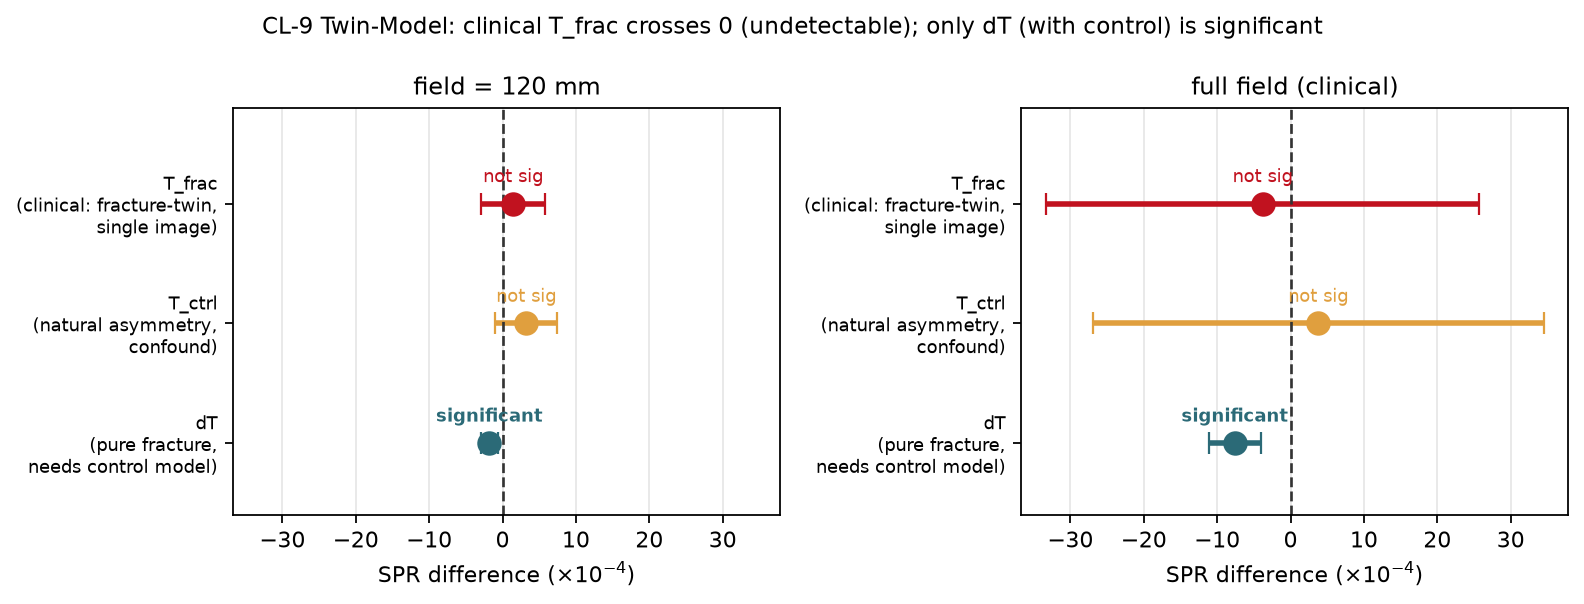
\includegraphics[width=0.98\textwidth]{fig/cl9_twin.png}
\caption{ค่าเฉลี่ย $\pm$ ช่วงความเชื่อมั่น 95\% ของ 3 ปริมาณ. \textbf{$T_{\text{frac}}$ (แดง) และ $T_{\text{ctrl}}$
(ส้ม) คร่อมเส้น 0} (ไม่มีนัยสำคัญ, error bar กว้าง โดยเฉพาะ full-field); เฉพาะ \textbf{$dT$ (น้ำเงิน) ไม่แตะ 0}
(significant) --- สัญญาณรอยแตกมีจริงแต่ ``จม'' อยู่ในความผันผวนของความไม่สมมาตร}
\end{figure}

\section{สรุปการทดสอบสมมติฐาน CL-9}
\begin{keybox}
\textbf{วิธี twin แบบตรงไปตรงมา:}\ \textcolor{bad}{$\boxtimes$ \textbf{ล้มเหลว (ที่ $N=10$)}} ---
ค่าที่แพทย์วัดได้ ($T_{\text{frac}}$) ไม่มีนัยสำคัญทั้งสองแบบสนาม เพราะ\textbf{ความไม่สมมาตรตามธรรมชาติ}
(ขนาดพอ ๆ กับสัญญาณ + ผันผวน seed-to-seed สูง) กลบรอยแตก\\[4pt]
\textbf{แต่มีความหวัง:} รอยแตกยัง\textbf{มีอยู่จริง} ($dT$ significant, $p<0.01$) และที่ full-field อัตราส่วน
$|dT|/|T_{\text{ctrl}}|=2.0$ = สัญญาณรอยแตกใหญ่กว่าความไม่สมมาตรเฉลี่ย 2 เท่า $\Rightarrow$
\textbf{ถ้าแก้/ลบความไม่สมมาตรออกได้ วิธี twin มีโอกาสใช้ได้}
\end{keybox}

\section{การตีความและงานถัดไป}
\begin{itemize}
  \item \textbf{ยืนยันการทำนายก่อนรัน:} ความไม่สมมาตร $\sim$1--2~มม.\ $>$ รอยแตก 0.5~มม.\ จริง --- จึงกลบสัญญาณ
        เหมือน confound ``mesh คนละก้อน'' ที่เคยฆ่าการทดลองแรก
  \item \textbf{ทำไม $T_{\text{frac}}$ จม:} การเทียบ 2 จุดที่อยู่ห่างกันบนภาพเดียว มี variance สูง (SPR ที่สองตำแหน่ง
        ผันผวนอิสระ) + ความไม่สมมาตรเพิ่ม bias --- ต่างจาก matched control ที่ใช้ common random numbers จึงสะอาด
  \item \textbf{งานถัดไป (ชี้จากผลนี้):} (ก)~\textbf{แก้ความไม่สมมาตร} ด้วย population template / baseline ของ
        คนไข้เอง / โมเดลเรียนรู้ความสมมาตรปกติ แล้วค่อยเทียบ twin; (ข)~เพิ่ม seed เพื่อวัดขนาด asymmetry ให้แม่น;
        (ค)~ทดสอบรอยแตกใหญ่ขึ้น ($>$1~มม.) ที่สัญญาณอาจชนะ asymmetry ได้เอง
\end{itemize}

\vfill
\noindent{\color{theme!45}\rule{\textwidth}{0.4pt}}\\
{\small\color{ink} รายงานเฉพาะ CL-9 (สมมติฐานเพิ่มเติมเชิงประยุกต์). ข้อมูล: 2 field settings $\times$ 10 seeds
(0.54~มม.). ดูรายงานอื่นที่ https://wwaxray.baanwit.com/doc/report/}

\end{document}
